\chapter{O ciclo celular e a mitose}\label{ch:g11:cell-cycle-mitosis}

Esmague a ponta de uma raiz de cebola sob uma lamínula, core o
material e olhe: entre centenas de \omterm{def:g10:cells-common-unit:cell}{células} tranquilas com \omterm{def:g10:cells-common-unit:organelle}{núcleo}
arredondado, algumas mostram outra coisa --- bastonetes escuros em
forma de X reunidos no meio da \omterm{def:g10:cells-common-unit:cell}{célula}, ou dois conjuntos de bastonetes
puxados para as extremidades, ou dois \omterm{def:g10:cells-common-unit:organelle}{núcleos} pequenos com uma parede
se formando entre eles. Você está vendo a divisão celular flagrada em
momentos diferentes, num tecido que cresce um milímetro por dia. Cada
uma dessas divisões entrega dois conjuntos completos e idênticos de
\omterm{def:g10:universal-dna:information}{cromossomos} a duas células-filhas. Este capítulo acompanha uma \omterm{def:g10:cells-common-unit:cell}{célula}
ao longo de um ciclo inteiro e observa de perto a hora em que os
\omterm{def:g10:universal-dna:information}{cromossomos} são repartidos.

\section{O ciclo celular}

\begin{definition}[Ciclo celular]\label{def:g11:cell-cycle-mitosis:cycle}
O \emph{ciclo celular}\index{ciclo celular} é a sequência de eventos
que vai do nascimento de uma \omterm{def:g10:cells-common-unit:cell}{célula}, por divisão, até a divisão dela
própria em duas. Ele compreende a \emph{interfase}, durante a qual a
\omterm{def:g10:cells-common-unit:cell}{célula} cresce e copia o \omterm{def:g10:universal-dna:information}{DNA} dela, e a \emph{fase M}, durante a qual o
\omterm{def:g10:cells-common-unit:organelle}{núcleo} se divide (a \emph{mitose}\index{mitose}) e em seguida o
\omterm{def:g10:cells-common-unit:cell}{citoplasma} (a \emph{citocinese}). A interfase tem três partes:
$\mathrm{G_1}$ (crescimento), S (a \omterm{def:g11:dna-replication:replication}{replicação do DNA},
\cref{ch:g11:dna-replication}) e $\mathrm{G_2}$ (preparação para a
divisão).
\end{definition}

\begin{omfigure}
\begin{tikzpicture}[font=\small]
  % pie: G1 11h, S 8h, G2 4h, M 1h  (24h) -> angles: G1 165°, S 120°, G2 60°, M 15°
  \fill[omDef!30] (0,0) -- (90:2.2) arc (90:-75:2.2) -- cycle;
  \fill[omProp!35] (0,0) -- (-75:2.2) arc (-75:-195:2.2) -- cycle;
  \fill[omMeth!35] (0,0) -- (-195:2.2) arc (-195:-255:2.2) -- cycle;
  \fill[omThm!50] (0,0) -- (-255:2.2) arc (-255:-270:2.2) -- cycle;
  \draw[thick] (0,0) circle (2.2);
  \foreach \a in {90,-75,-195,-255} \draw[thick] (0,0) -- (\a:2.2);
  \node at (10:1.3) {$\mathrm{G_1}$};
  \node at (-135:1.3) {S};
  \node at (-225:1.35) {$\mathrm{G_2}$};
  \node[anchor=south east] at (-262:2.35) {M};
  \node[anchor=west, align=left] at (2.6,1.3) {$\mathrm{G_1}$: crescimento, cerca de \qty{11}{h}};
  \node[anchor=west, align=left] at (2.6,0.5) {S: replicação do DNA, \qty{8}{h}};
  \node[anchor=west, align=left] at (2.6,-0.3) {$\mathrm{G_2}$: preparação, \qty{4}{h}};
  \node[anchor=west, align=left] at (2.6,-1.1) {M: mitose e citocinese, \qty{1}{h}};
  \draw[->, thick] (100:2.5) arc (100:130:2.5);
\end{tikzpicture}

{\small O \omterm{def:g11:cell-cycle-mitosis:cycle}{ciclo celular} de uma \omterm{def:g10:cells-common-unit:cell}{célula} humana em divisão típica, cerca
de 24 horas. A interfase ($\mathrm{G_1}$, S, $\mathrm{G_2}$) ocupa 23
delas; a divisão em si, uma. Muitas \omterm{def:g10:cells-common-unit:cell}{células} saem do ciclo depois de
$\mathrm{G_1}$ e nunca mais se dividem.}
\end{omfigure}

\begin{proposition}[O DNA ao longo do ciclo]\label{prop:g11:cell-cycle-mitosis:dna}
Chame de $q$ a quantidade de \omterm{def:g10:universal-dna:information}{DNA} de um \omterm{def:g10:cells-common-unit:organelle}{núcleo} logo depois da divisão.
Ela fica em $q$ ao longo de $\mathrm{G_1}$, sobe com regularidade até
$2q$ durante S à medida que os \omterm{def:g10:universal-dna:information}{cromossomos} são copiados, fica em $2q$
ao longo de $\mathrm{G_2}$ e da primeira parte da \omterm{def:g11:cell-cycle-mitosis:cycle}{mitose}, e volta a $q$
em cada núcleo-filho no fim da \omterm{def:g11:cell-cycle-mitosis:cycle}{mitose}. O número de \omterm{def:g10:universal-dna:information}{cromossomos} não muda
durante S: cada \omterm{def:g11:cell-cycle-mitosis:chromosome}{cromossomo} é copiado em duas \emph{\omterm{def:g11:cell-cycle-mitosis:chromosome}{cromátides}}
idênticas mantidas juntas pelo \emph{\omterm{def:g11:cell-cycle-mitosis:chromosome}{centrômero}} delas, e só se separa
em dois \omterm{def:g10:universal-dna:information}{cromossomos} durante a \omterm{def:g11:cell-cycle-mitosis:cycle}{mitose}.
\end{proposition}
\admitted

\begin{omfigure}
\begin{tikzpicture}
\begin{axis}[
  width=0.9\linewidth, height=5.4cm,
  axis x line=bottom, axis y line=left,
  xmin=0, xmax=50, ymin=0, ymax=2.8,
  xlabel={tempo (h)}, ylabel={DNA por núcleo},
  xlabel style={font=\small, at={(axis description cs:0.5,-0.1)}, anchor=north},
  ylabel style={font=\small},
  tick label style={font=\small}, xtick={0,11,19,23,24,35,43,47,48},
  xticklabels={0,11,19,23,,24,35,43,,48},
  ytick={1,2}, yticklabels={$q$, $2q$},
  clip=false,
]
\addplot[thick, omDef] coordinates {(0,1) (11,1) (19,2) (23,2) (23.9,2) (24,1) (35,1) (43,2) (47,2) (47.9,2) (48,1) (50,1)};
\node[font=\small, anchor=south] at (axis cs:5.5,2.25) {$\mathrm{G_1}$};
\node[font=\small, anchor=south] at (axis cs:15,2.25) {S};
\node[font=\small, anchor=south] at (axis cs:21,2.25) {$\mathrm{G_2}$};
\node[font=\small, anchor=south] at (axis cs:29.5,2.25) {$\mathrm{G_1}$};
\node[font=\small, anchor=south] at (axis cs:39,2.25) {S};
\node[font=\small, anchor=south] at (axis cs:45,2.25) {$\mathrm{G_2}$};
\node[font=\small, anchor=south, omThm] at (axis cs:23.5,2.55) {M};
\node[font=\small, anchor=south, omThm] at (axis cs:47.5,2.55) {M};
\draw[dashed, gray] (axis cs:11,0) -- (axis cs:11,2.2);
\draw[dashed, gray] (axis cs:19,0) -- (axis cs:19,2.2);
\draw[dashed, gray] (axis cs:23,0) -- (axis cs:23,2.2);
\draw[dashed, gray] (axis cs:24,0) -- (axis cs:24,2.2);
\draw[dashed, gray] (axis cs:35,0) -- (axis cs:35,2.2);
\draw[dashed, gray] (axis cs:43,0) -- (axis cs:43,2.2);
\draw[dashed, gray] (axis cs:47,0) -- (axis cs:47,2.2);
\end{axis}
\end{tikzpicture}

{\small Quantidade de \omterm{def:g10:universal-dna:information}{DNA} de um \omterm{def:g10:cells-common-unit:organelle}{núcleo} ao longo de dois ciclos
sucessivos de 24 horas. Ela dobra durante S e cai pela metade no fim da
\omterm{def:g11:cell-cycle-mitosis:cycle}{mitose}; uma célula-filha sempre começa com $q$.}
\end{omfigure}

\begin{example}[Ler a curva]\label{ex:g11:cell-cycle-mitosis:reading}
Uma \omterm{def:g10:cells-common-unit:cell}{célula} medida em $2q$ pode estar em $\mathrm{G_2}$ ou no início da
\omterm{def:g11:cell-cycle-mitosis:cycle}{mitose}; em $1.5q$ ela está com certeza em S, na metade da replicação;
em $q$ ela está em $\mathrm{G_1}$ --- ou saiu do ciclo de vez, como um
neurônio ou uma fibra muscular, que ficam em $q$ a vida toda. Um tecido
em que toda \omterm{def:g10:cells-common-unit:cell}{célula} está em $q$ é um tecido que parou de se dividir.
\end{example}

\section{Os cromossomos, vistos}

\begin{definition}[Cromossomo, cromátide, cariótipo]\label{def:g11:cell-cycle-mitosis:chromosome}
Um \emph{cromossomo} é uma molécula de \omterm{def:g10:universal-dna:information}{DNA} com as \omterm{def:g10:chemistry-of-life:families}{proteínas} de
empacotamento dela. Entre duas divisões ele é um fio frouxo e
invisível; no início da \omterm{def:g11:cell-cycle-mitosis:cycle}{mitose} ele se espirala num bastonete compacto
visível ao microscópio ótico. Depois da replicação cada cromossomo é
formado por duas \emph{cromátides}\index{cromátide} idênticas, unidas
pelo \emph{centrômero}\index{centrômero}: a forma de X familiar. O
\emph{cariótipo}\index{cariótipo} de uma \omterm{def:g10:biodiversity-scales:species}{espécie} é o conjunto completo
de \omterm{def:g10:universal-dna:information}{cromossomos} dela, fotografado em metáfase e arrumado em pares por
tamanho: uma \omterm{def:g10:cells-common-unit:cell}{célula} humana tem 46, em 23 pares, sendo os membros de um
par \emph{homólogos} --- mesmos \omterm{def:g10:universal-dna:gene}{genes} nas mesmas posições, um de cada
genitor.
\end{definition}

\begin{omfigure}
\begin{tikzpicture}[font=\scriptsize, line cap=round]
  % 22 autosome pairs of decreasing size, then X and Y; each chromosome = two chromatids
  \tikzset{chrom/.style={line width=2.6pt, omDef!75}}
  \foreach \n/\h/\c in {1/2.4/0.55, 2/2.3/0.5, 3/2.0/0.5, 4/1.9/0.35, 5/1.8/0.35, 6/1.7/0.45, 7/1.55/0.42, 8/1.45/0.4}
    { \pgfmathsetmacro{\x}{(\n-1)*1.55}
      \draw[chrom] (\x,0) -- (\x,\h); \draw[chrom] (\x+0.22,0) -- (\x+0.22,\h);
      \fill[omThm] (\x+0.11,{\h*\c}) circle (2pt);
      \node[anchor=north] at (\x+0.11,-0.08) {\n}; }
  \foreach \n/\h/\c in {9/1.4/0.35, 10/1.35/0.35, 11/1.35/0.4, 12/1.3/0.3, 13/1.1/0.15, 14/1.05/0.15, 15/1.0/0.15, 16/0.9/0.45}
    { \pgfmathsetmacro{\x}{(\n-9)*1.55}
      \draw[chrom] (\x,-3.2) -- (\x,-3.2+\h); \draw[chrom] (\x+0.22,-3.2) -- (\x+0.22,-3.2+\h);
      \fill[omThm] (\x+0.11,{-3.2+\h*\c}) circle (2pt);
      \node[anchor=north] at (\x+0.11,-3.28) {\n}; }
  \foreach \n/\h/\c in {17/0.85/0.3, 18/0.8/0.2, 19/0.65/0.5, 20/0.65/0.5, 21/0.5/0.2, 22/0.5/0.2}
    { \pgfmathsetmacro{\x}{(\n-17)*1.55}
      \draw[chrom] (\x,-5.6) -- (\x,-5.6+\h); \draw[chrom] (\x+0.22,-5.6) -- (\x+0.22,-5.6+\h);
      \fill[omThm] (\x+0.11,{-5.6+\h*\c}) circle (2pt);
      \node[anchor=north] at (\x+0.11,-5.68) {\n}; }
  % sex chromosomes
  \draw[chrom] (9.3,-5.6) -- (9.3,-4.1); \draw[chrom] (9.52,-5.6) -- (9.52,-4.1); \fill[omThm] (9.41,-4.85) circle (2pt);
  \node[anchor=north] at (9.41,-5.68) {X};
  \draw[chrom] (10.85,-5.6) -- (10.85,-5.1); \draw[chrom] (11.07,-5.6) -- (11.07,-5.1); \fill[omThm] (10.96,-5.5) circle (2pt);
  \node[anchor=north] at (10.96,-5.68) {Y};
\end{tikzpicture}

{\small Um \omterm{def:g11:cell-cycle-mitosis:chromosome}{cariótipo} humano, esquematicamente: os 22 pares de
\omterm{def:g10:universal-dna:information}{cromossomos} comuns numerados por tamanho decrescente, depois os
\omterm{def:g10:universal-dna:information}{cromossomos} sexuais --- X e Y aqui, logo um homem. Cada \omterm{def:g11:cell-cycle-mitosis:chromosome}{cromossomo} está
desenhado como as duas \omterm{def:g11:cell-cycle-mitosis:chromosome}{cromátides} dele, com o \omterm{def:g11:cell-cycle-mitosis:chromosome}{centrômero} em vermelho.}
\end{omfigure}

\begin{omfigure}
\begin{tikzpicture}[font=\small, line cap=round]
  % single chromatid chromosome
  \draw[line width=5pt, omDef!70] (0,-1.2) -- (0,1.2);
  \fill[omThm] (0,0.2) circle (3.5pt);
  \node[anchor=north, align=center] at (0,-1.5) {antes da fase S:\\ uma cromátide};
  % arrow
  \draw[->, thick] (1.2,0) -- (2.6,0) node[midway, above] {S};
  % two chromatid chromosome
  \draw[line width=5pt, omDef!70] (3.6,-1.2) .. controls (3.75,-0.3) and (3.75,0.3) .. (3.6,1.2);
  \draw[line width=5pt, omDef!70] (4.2,-1.2) .. controls (4.05,-0.3) and (4.05,0.3) .. (4.2,1.2);
  \fill[omThm] (3.9,0.2) circle (3.5pt);
  \node[anchor=north, align=center] at (3.9,-1.5) {depois da fase S:\\ duas cromátides idênticas};
  \draw[->] (5.6,0.2) -- (4.15,0.2) node[pos=0, anchor=west] {centrômero};
  \draw[->] (5.6,0.9) -- (4.35,0.9) node[pos=0, anchor=west] {cromátide};
  % after anaphase
  \draw[->, thick] (8.6,0) -- (10.0,0) node[midway, above] {anáfase};
  \draw[line width=5pt, omDef!70] (10.8,-1.2) -- (10.8,1.2);
  \fill[omThm] (10.8,0.2) circle (3.5pt);
  \draw[line width=5pt, omDef!70] (11.8,-1.2) -- (11.8,1.2);
  \fill[omThm] (11.8,0.2) circle (3.5pt);
  \node[anchor=north, align=center] at (11.3,-1.5) {dois cromossomos,\\ um para cada célula};
\end{tikzpicture}

{\small Um \omterm{def:g11:cell-cycle-mitosis:chromosome}{cromossomo} ao longo do ciclo. A replicação o transforma em
duas \omterm{def:g11:cell-cycle-mitosis:chromosome}{cromátides} unidas pelo \omterm{def:g11:cell-cycle-mitosis:chromosome}{centrômero}; a anáfase as separa em dois
\omterm{def:g10:universal-dna:information}{cromossomos} de uma \omterm{def:g11:cell-cycle-mitosis:chromosome}{cromátide} cada, um para cada célula-filha. A
contagem de \omterm{def:g10:universal-dna:information}{cromossomos} só muda na anáfase.}
\end{omfigure}

\section{A mitose, passo a passo}

\begin{proposition}[As quatro etapas da mitose]\label{prop:g11:cell-cycle-mitosis:stages}
A \omterm{def:g11:cell-cycle-mitosis:cycle}{mitose} é um movimento contínuo, descrito em quatro etapas.
\begin{enumerate}
  \item \emph{Prófase}: os \omterm{def:g10:universal-dna:information}{cromossomos} se condensam em bastonetes
        visíveis de duas \omterm{def:g11:cell-cycle-mitosis:chromosome}{cromátides}; o envoltório nuclear se desfaz;
        um \emph{fuso} de fibras de \omterm{def:g10:chemistry-of-life:families}{proteína} se forma entre os dois
        polos da \omterm{def:g10:cells-common-unit:cell}{célula}.
  \item \emph{Metáfase}: os \omterm{def:g10:universal-dna:information}{cromossomos}, presos às fibras do fuso
        pelos \omterm{def:g11:cell-cycle-mitosis:chromosome}{centrômeros} deles, se alinham no plano equatorial da
        \omterm{def:g10:cells-common-unit:cell}{célula}.
  \item \emph{Anáfase}: os \omterm{def:g11:cell-cycle-mitosis:chromosome}{centrômeros} se dividem; as duas \omterm{def:g11:cell-cycle-mitosis:chromosome}{cromátides}
        de cada \omterm{def:g11:cell-cycle-mitosis:chromosome}{cromossomo}, agora dois \omterm{def:g10:universal-dna:information}{cromossomos}, são puxadas para
        polos opostos pelas fibras que encurtam.
  \item \emph{Telófase}: um envoltório nuclear se refaz em torno de
        cada conjunto; os \omterm{def:g10:universal-dna:information}{cromossomos} se desespiralam. A citocinese
        divide então o \omterm{def:g10:cells-common-unit:cell}{citoplasma} --- por estrangulamento nas \omterm{def:g10:cells-common-unit:cell}{células}
        animais, construindo uma nova parede nas \omterm{def:g10:cells-common-unit:cell}{células} vegetais.
\end{enumerate}
Cada célula-filha recebe uma \omterm{def:g11:cell-cycle-mitosis:chromosome}{cromátide} de cada \omterm{def:g11:cell-cycle-mitosis:chromosome}{cromossomo}: o mesmo
número de \omterm{def:g10:universal-dna:information}{cromossomos} da mãe, carregando o mesmo \omterm{def:g10:universal-dna:information}{DNA}.
\end{proposition}
\admitted

\begin{omfigure}
\begin{tikzpicture}[font=\small, line cap=round]
  \tikzset{cellb/.style={draw, thick, fill=omDef!5, rounded corners=10pt, minimum width=2.9cm, minimum height=2.6cm},
           chr/.style={line width=3pt, omDef!80}, cen/.style={fill=omThm}}
  % prophase
  \begin{scope}
    \node[cellb] at (0,0) {};
    \draw[thick, dashed, gray] (0,0) circle (0.95);
    \draw[chr] (-0.5,0.5) .. controls (-0.35,0.1) .. (-0.5,-0.3); \draw[chr] (-0.2,0.5) .. controls (-0.35,0.1) .. (-0.2,-0.3); \fill[cen] (-0.35,0.1) circle (2pt);
    \draw[chr] (0.2,0.6) .. controls (0.35,0.2) .. (0.2,-0.2); \draw[chr] (0.5,0.6) .. controls (0.35,0.2) .. (0.5,-0.2); \fill[cen] (0.35,0.2) circle (2pt);
    \node[anchor=north, align=center] at (0,-1.45) {prófase};
  \end{scope}
  % metaphase
  \begin{scope}[xshift=3.6cm]
    \node[cellb] at (0,0) {};
    \fill (0,1.1) circle (2pt); \fill (0,-1.1) circle (2pt);
    \foreach \x in {-0.45,0.45} { \draw[gray] (0,1.1) -- (\x,0.05); \draw[gray] (0,-1.1) -- (\x,-0.05); }
    \foreach \x in {-0.45,0.45} {
      \draw[chr] (\x-0.13,0.55) .. controls (\x,0.0) .. (\x-0.13,-0.55);
      \draw[chr] (\x+0.13,0.55) .. controls (\x,0.0) .. (\x+0.13,-0.55);
      \fill[cen] (\x,0) circle (2pt);
    }
    \draw[dashed, gray] (-1.3,0) -- (1.3,0);
    \node[anchor=north, align=center] at (0,-1.45) {metáfase};
  \end{scope}
  % anaphase
  \begin{scope}[xshift=7.2cm]
    \node[cellb] at (0,0) {};
    \fill (0,1.1) circle (2pt); \fill (0,-1.1) circle (2pt);
    \foreach \x in {-0.45,0.45} { \draw[gray] (0,1.1) -- (\x,0.6); \draw[gray] (0,-1.1) -- (\x,-0.6); }
    \foreach \x in {-0.45,0.45} {
      \draw[chr] (\x,0.6) .. controls (\x-0.1,0.4) .. (\x-0.25,0.05);
      \draw[chr] (\x,0.6) .. controls (\x+0.1,0.4) .. (\x+0.25,0.05);
      \fill[cen] (\x,0.6) circle (2pt);
      \draw[chr] (\x,-0.6) .. controls (\x-0.1,-0.4) .. (\x-0.25,-0.05);
      \draw[chr] (\x,-0.6) .. controls (\x+0.1,-0.4) .. (\x+0.25,-0.05);
      \fill[cen] (\x,-0.6) circle (2pt);
    }
    \node[anchor=north, align=center] at (0,-1.45) {anáfase};
  \end{scope}
  % telophase
  \begin{scope}[xshift=10.8cm]
    \draw[thick, fill=omDef!5] (-1.45,1.3) .. controls (-1.6,0.3) and (-0.3,0.3) .. (0,0) .. controls (-0.3,-0.3) and (-1.6,-0.3) .. (-1.45,-1.3) -- cycle;
    \draw[thick, fill=omDef!5] (1.45,1.3) .. controls (1.6,0.3) and (0.3,0.3) .. (0,0) .. controls (0.3,-0.3) and (1.6,-0.3) .. (1.45,-1.3) -- cycle;
    \draw[thick, fill=omDef!5, rounded corners=10pt] (-1.45,-1.3) rectangle (1.45,1.3);
    \draw[thick, fill=white] (-1.45,1.3) .. controls (-1.6,0.3) and (-0.3,0.3) .. (0,0) .. controls (-0.3,-0.3) and (-1.6,-0.3) .. (-1.45,-1.3);
    \draw[thick, fill=white] (1.45,1.3) .. controls (1.6,0.3) and (0.3,0.3) .. (0,0) .. controls (0.3,-0.3) and (1.6,-0.3) .. (1.45,-1.3);
    \draw[thick, dashed, gray] (-0.75,0) circle (0.5); \draw[thick, dashed, gray] (0.75,0) circle (0.5);
    \foreach \x in {-0.9,-0.6,0.6,0.9} \draw[chr] (\x,0.25) -- (\x,-0.25);
    \node[anchor=north, align=center] at (0,-1.45) {telófase e\\ citocinese};
  \end{scope}
\end{tikzpicture}

{\small \omterm{def:g11:cell-cycle-mitosis:cycle}{Mitose} de uma \omterm{def:g10:cells-common-unit:cell}{célula} com dois \omterm{def:g10:universal-dna:information}{cromossomos} ($2n = 2$), cada um
já formado por duas \omterm{def:g11:cell-cycle-mitosis:chromosome}{cromátides}. Prófase: condensação, envoltório
desfeito. Metáfase: alinhamento no equador, \omterm{def:g11:cell-cycle-mitosis:chromosome}{centrômeros} presos ao
fuso. Anáfase: \omterm{def:g11:cell-cycle-mitosis:chromosome}{cromátides} puxadas para os polos. Telófase: dois \omterm{def:g10:cells-common-unit:organelle}{núcleos}
se refazem e a \omterm{def:g10:cells-common-unit:cell}{célula} se divide.}
\end{omfigure}

\begin{omfigure}
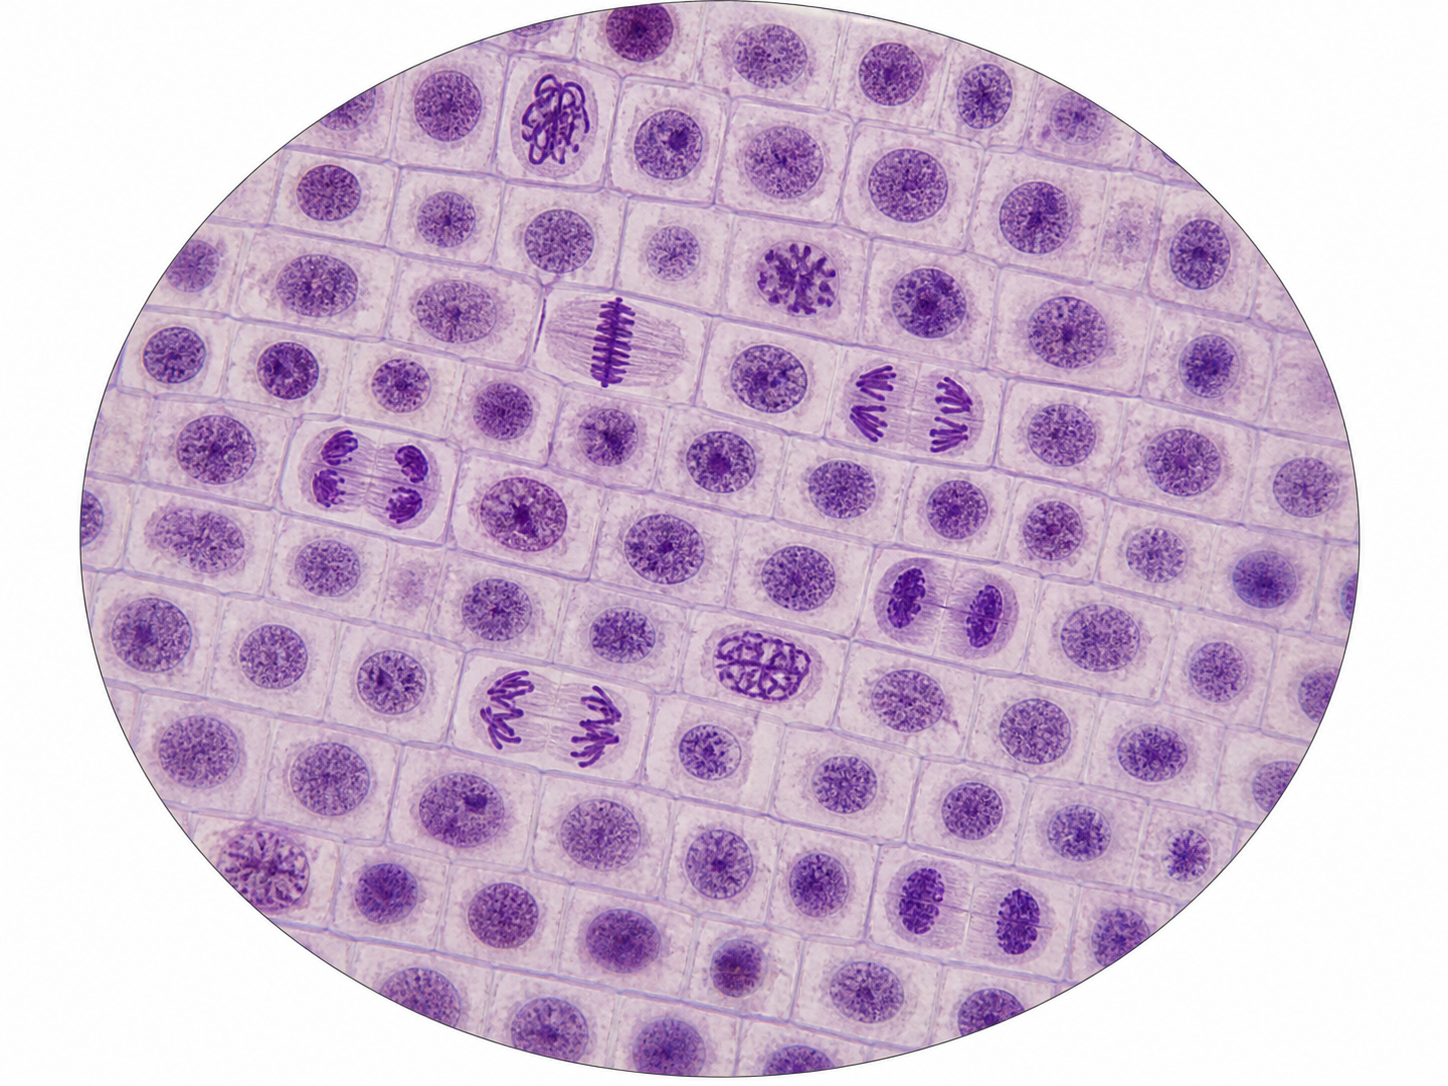
\includegraphics[width=0.58\linewidth]{images/book2/ai/g11-mitosis-root-tip.png}

{\small Um esmagamento de ponta de raiz de cebola ao microscópio
ótico. A maior parte das \omterm{def:g10:cells-common-unit:cell}{células} está em interfase; algumas mostram
\omterm{def:g10:universal-dna:information}{cromossomos} condensados em etapas diferentes da \omterm{def:g11:cell-cycle-mitosis:cycle}{mitose}. Contar a
proporção em cada etapa mede quanto dura cada uma delas.}
\end{omfigure}

\begin{example}[Contar na ponta da raiz]\label{ex:g11:cell-cycle-mitosis:count}
De 600 \omterm{def:g10:cells-common-unit:cell}{células} contadas numa ponta de raiz, 540 estão em interfase e 60
em \omterm{def:g11:cell-cycle-mitosis:cycle}{mitose}: um \emph{índice mitótico} de 10\%. Se o ciclo dura 20 horas,
a \omterm{def:g11:cell-cycle-mitosis:cycle}{mitose} dura cerca de $0.10 \times 20 = \qty{2}{h}$; e se 36 das 60
\omterm{def:g10:cells-common-unit:cell}{células} em divisão estão em prófase, a prófase ocupa $36/60$ dessas
duas horas, uns 72 minutos, enquanto a anáfase, vista em apenas 4
\omterm{def:g10:cells-common-unit:cell}{células}, leva cerca de 8 minutos. A etapa mais rara é a mais rápida.
\end{example}

\begin{method}[Contar cromossomos e cromátides]\label{met:g11:cell-cycle-mitosis:counting}
Para uma \omterm{def:g10:biodiversity-scales:species}{espécie} com $2n$ \omterm{def:g10:universal-dna:information}{cromossomos}:
\begin{enumerate}
  \item em $\mathrm{G_1}$: $2n$ \omterm{def:g10:universal-dna:information}{cromossomos}, uma \omterm{def:g11:cell-cycle-mitosis:chromosome}{cromátide} cada, \omterm{def:g10:universal-dna:information}{DNA}
        $q$;
  \item depois de S, ao longo de $\mathrm{G_2}$, da prófase e da
        metáfase: $2n$ \omterm{def:g10:universal-dna:information}{cromossomos}, duas \omterm{def:g11:cell-cycle-mitosis:chromosome}{cromátides} cada ($4n$
        \omterm{def:g11:cell-cycle-mitosis:chromosome}{cromátides}), \omterm{def:g10:universal-dna:information}{DNA} $2q$;
  \item a partir da anáfase: $4n$ \omterm{def:g10:universal-dna:information}{cromossomos} de uma \omterm{def:g11:cell-cycle-mitosis:chromosome}{cromátide} na
        \omterm{def:g10:cells-common-unit:cell}{célula}, $2n$ indo para cada polo;
  \item em cada célula-filha: $2n$ \omterm{def:g10:universal-dna:information}{cromossomos}, uma \omterm{def:g11:cell-cycle-mitosis:chromosome}{cromátide} cada,
        \omterm{def:g10:universal-dna:information}{DNA} $q$.
\end{enumerate}
Uma \omterm{def:g11:cell-cycle-mitosis:chromosome}{cromátide} vira um \omterm{def:g11:cell-cycle-mitosis:chromosome}{cromossomo} no instante em que o \omterm{def:g11:cell-cycle-mitosis:chromosome}{centrômero} dela
se divide.
\end{method}

\begin{example}[Os números humanos]\label{ex:g11:cell-cycle-mitosis:human}
Uma \omterm{def:g10:cells-common-unit:cell}{célula} humana em metáfase tem 46 \omterm{def:g10:universal-dna:information}{cromossomos} e 92 \omterm{def:g11:cell-cycle-mitosis:chromosome}{cromátides}; em
anáfase, 92 \omterm{def:g10:universal-dna:information}{cromossomos}, 46 indo para cada polo; cada filha, 46
\omterm{def:g10:universal-dna:information}{cromossomos} de uma \omterm{def:g11:cell-cycle-mitosis:chromosome}{cromátide} cada, contendo exatamente o \omterm{def:g10:universal-dna:information}{DNA} que a mãe
tinha no início do ciclo dela.
\end{example}

\section{Para que serve a mitose}

\begin{proposition}[Conformidade e usos dela]\label{prop:g11:cell-cycle-mitosis:conformity}
Como a replicação é fiel e a \omterm{def:g11:cell-cycle-mitosis:cycle}{mitose} distribui as \omterm{def:g11:cell-cycle-mitosis:chromosome}{cromátides}
exatamente, toda \omterm{def:g10:cells-common-unit:cell}{célula} de um corpo pluricelular carrega a mesma
\omterm{def:g10:universal-dna:information}{informação genética} do óvulo fecundado de que ela descende. A \omterm{def:g11:cell-cycle-mitosis:cycle}{mitose} é
o mecanismo do crescimento (o embrião, a ponta da raiz), da renovação
(pele, revestimento do intestino, sangue: só a medula óssea fabrica uns
$\num{2e11}$ \omterm{def:g10:cells-common-unit:cell}{células} por dia) e do reparo (a cicatrização de feridas);
nos eucariontes unicelulares ela é a própria reprodução. O controle
dela --- a decisão de entrar no ciclo, as conferências antes de S e
antes da anáfase --- é assunto do \cref{ch:g11:cancer}.
\end{proposition}
\admitted

\begin{remark}[Nem tudo se divide]\label{rem:g11:cell-cycle-mitosis:notall}
A maioria dos neurônios e das \omterm{def:g10:cells-common-unit:cell}{células} musculares do coração sai do
ciclo no início da infância e nunca mais volta a entrar nele: o dano a
elas não é reparado por divisão, e é por isso que uma lesão da medula
espinal ou um infarto deixam perda duradoura. As \omterm{def:g10:cells-common-unit:cell}{células} do fígado
repousam em $\mathrm{G_1}$ por meses, mas voltam ao ciclo quando parte
do fígado é retirada, refazendo o órgão em poucas semanas. Que \omterm{def:g10:cells-common-unit:cell}{células}
podem se dividir, e quando, é uma das regulações mais estritas do
corpo.
\end{remark}

\section{Exercícios}

\begin{exercise}[$\star$]\label{exo:g11:cell-cycle-mitosis:1}
Cite as quatro fases do \omterm{def:g11:cell-cycle-mitosis:cycle}{ciclo celular} e diga o que acontece em cada uma.
\end{exercise}

\begin{exercise}[$\star$]\label{exo:g11:cell-cycle-mitosis:2}
Defina \omterm{def:g11:cell-cycle-mitosis:chromosome}{cromátide} e \omterm{def:g11:cell-cycle-mitosis:chromosome}{centrômero}. Quando um \omterm{def:g11:cell-cycle-mitosis:chromosome}{cromossomo} tem duas
\omterm{def:g11:cell-cycle-mitosis:chromosome}{cromátides}?
\end{exercise}

\begin{exercise}[$\star$]\label{exo:g11:cell-cycle-mitosis:3}
Liste as quatro etapas da \omterm{def:g11:cell-cycle-mitosis:cycle}{mitose} com um evento-chave em cada uma.
\end{exercise}

\begin{exercise}[$\star$]\label{exo:g11:cell-cycle-mitosis:4}
Um \omterm{def:g10:cells-common-unit:organelle}{núcleo} contém $1.5q$ de \omterm{def:g10:universal-dna:information}{DNA}. Em que fase está a \omterm{def:g10:cells-common-unit:cell}{célula}?
\end{exercise}

\begin{exercise}[$\star$]\label{exo:g11:cell-cycle-mitosis:5}
Quantos \omterm{def:g10:universal-dna:information}{cromossomos}, e quantas \omterm{def:g11:cell-cycle-mitosis:chromosome}{cromátides}, tem uma \omterm{def:g10:cells-common-unit:cell}{célula} humana em
$\mathrm{G_2}$?
\end{exercise}

\begin{exercise}[$\star\star$]\label{exo:g11:cell-cycle-mitosis:6}
A partir da figura da quantidade de \omterm{def:g10:universal-dna:information}{DNA}, dê a duração de cada fase e
diga em que fases uma \omterm{def:g10:cells-common-unit:cell}{célula} seria encontrada com $2q$.
\end{exercise}

\begin{exercise}[$\star\star$]\label{exo:g11:cell-cycle-mitosis:7}
Um camundongo tem $2n = 40$. Dê o número de \omterm{def:g10:universal-dna:information}{cromossomos} e de \omterm{def:g11:cell-cycle-mitosis:chromosome}{cromátides}
numa \omterm{def:g10:cells-common-unit:cell}{célula} em metáfase, em anáfase (\omterm{def:g10:cells-common-unit:cell}{célula} inteira) e numa
célula-filha.
\end{exercise}

\begin{exercise}[$\star\star$]\label{exo:g11:cell-cycle-mitosis:8}
Numa ponta de raiz, 800 \omterm{def:g10:cells-common-unit:cell}{células} são contadas: 720 em interfase, 48 em
prófase, 16 em metáfase, 6 em anáfase, 10 em telófase. Calcule o índice
mitótico e, para um ciclo de 24 horas, a duração de cada etapa.
\end{exercise}

\begin{exercise}[$\star\star$]\label{exo:g11:cell-cycle-mitosis:9}
A colchicina, um medicamento extraído do cólquico, impede o fuso de se
formar. Preveja o que acontece a uma \omterm{def:g10:cells-common-unit:cell}{célula} em divisão tratada com ela,
e por que os biólogos a usam para preparar \omterm{def:g11:cell-cycle-mitosis:chromosome}{cariótipos}.
\end{exercise}

\begin{exercise}[$\star\star$]\label{exo:g11:cell-cycle-mitosis:10}
Explique por que os \omterm{def:g10:universal-dna:information}{cromossomos} precisam se condensar antes de serem
movidos, e por que eles se desespiralam de novo depois.
\end{exercise}

\begin{exercise}[$\star\star$]\label{exo:g11:cell-cycle-mitosis:11}
Um óvulo fecundado se divide a cada 12 horas nos primeiros dias.
Quantas \omterm{def:g10:cells-common-unit:cell}{células} existem depois de 5 dias? Cada divisão precisaria de um
$\mathrm{G_1}$ completo?
\end{exercise}

\begin{exercise}[$\star\star\star$]\label{exo:g11:cell-cycle-mitosis:12}
Na anáfase, as duas \omterm{def:g11:cell-cycle-mitosis:chromosome}{cromátides} de um \omterm{def:g11:cell-cycle-mitosis:chromosome}{cromossomo} não conseguem se
separar e as duas vão para o mesmo polo. Descreva as duas células-filhas
(número de \omterm{def:g10:universal-dna:information}{cromossomos}, \omterm{def:g10:universal-dna:information}{DNA}) e explique por que um erro desses, numa
\omterm{def:g10:cells-common-unit:cell}{célula} do corpo, em geral não tem consequência, mas em alguns casos é
grave.
\end{exercise}

\begin{exercise}[$\star\star\star$]\label{exo:g11:cell-cycle-mitosis:13}
A medula óssea fabrica $\num{2e11}$ \omterm{def:g10:cells-common-unit:cell}{células} sanguíneas por dia. Se uma
\omterm{def:g10:cells-common-unit:cell}{célula} precursora da medula completa um ciclo em 24 horas, estime
quantas precursoras estão se dividindo a cada instante, e comente o que
um medicamento que bloqueie a \omterm{def:g11:cell-cycle-mitosis:cycle}{mitose} faria com o sangue em uma semana.
\end{exercise}

\begin{exercise}[$\star\star\star$]\label{exo:g11:cell-cycle-mitosis:14}
Explique por que um \omterm{def:g11:cell-cycle-mitosis:chromosome}{cariótipo} é preparado a partir de \omterm{def:g10:cells-common-unit:cell}{células} paradas
em metáfase, e não em interfase ou em anáfase.
\end{exercise}

\begin{exercise}[$\star\star\star$]\label{exo:g11:cell-cycle-mitosis:15}
Um fígado é retirado em dois terços; em três semanas ele voltou a
crescer. Usando o \omterm{def:g11:cell-cycle-mitosis:cycle}{ciclo celular}, descreva o que as \omterm{def:g10:cells-common-unit:cell}{células} dele
fizeram, e diga como era o conteúdo em \omterm{def:g10:universal-dna:information}{DNA} das \omterm{def:g10:cells-common-unit:cell}{células} do fígado no dia
3 comparado com o dia 0.
\end{exercise}

\section{Problema: o cronograma da ponta da raiz}

\begin{problem}[{Problema de fim de semana --- uma ponta de raiz contada
célula a célula: a duração de cada etapa do ciclo, o DNA a cada momento,
as células que uma raiz fabrica num dia, e os oito minutos da anáfase}]
\label{pb:g11:cell-cycle-mitosis:1}
Uma turma esmaga e cora a ponta de uma raiz de alho ($2n = 16$) e conta
1000 \omterm{def:g10:cells-common-unit:cell}{células} na zona de crescimento: 900 em interfase, 60 em prófase,
18 em metáfase, 8 em anáfase, 14 em telófase. Medidas independentes dão
o ciclo dessas \omterm{def:g10:cells-common-unit:cell}{células} como 20 horas. Tome a zona de crescimento como
contendo 20\,000 \omterm{def:g10:cells-common-unit:cell}{células}.

\medskip
\noindent\textbf{Parte I --- O índice mitótico.}
\begin{enumerate}
  \item Calcule o índice mitótico do tecido.
  \item Supondo que a fração de \omterm{def:g10:cells-common-unit:cell}{células} numa etapa seja igual à fração
        do ciclo passada nela, calcule a duração da \omterm{def:g11:cell-cycle-mitosis:cycle}{mitose}.
  \item Calcule a duração de cada uma das quatro etapas.
  \item Que etapa é a mais curta? Sugira por que ela pode ser tão
        rápida.
  \item Por que o método exige contar muitas \omterm{def:g10:cells-common-unit:cell}{células}, e por que elas
        precisam vir apenas da zona de crescimento?
\end{enumerate}

\medskip
\noindent\textbf{Parte II --- \omterm{def:g10:universal-dna:information}{Cromossomos} e \omterm{def:g10:universal-dna:information}{DNA}.}
\begin{enumerate}[resume]
  \item Quantos \omterm{def:g10:universal-dna:information}{cromossomos}, e quantas \omterm{def:g11:cell-cycle-mitosis:chromosome}{cromátides}, tem uma \omterm{def:g10:cells-common-unit:cell}{célula} de
        alho em metáfase?
  \item Quantos \omterm{def:g10:universal-dna:information}{cromossomos} estão se movendo numa \omterm{def:g10:cells-common-unit:cell}{célula} em anáfase, e
        quantos chegam a cada polo?
  \item Chamando de $q$ o \omterm{def:g10:universal-dna:information}{DNA} de uma célula-filha, dê o conteúdo em \omterm{def:g10:universal-dna:information}{DNA}
        de uma \omterm{def:g10:cells-common-unit:cell}{célula} em prófase, em anáfase (\omterm{def:g10:cells-common-unit:cell}{célula} inteira) e em
        telófase (cada \omterm{def:g10:cells-common-unit:organelle}{núcleo}).
  \item Das 900 \omterm{def:g10:cells-common-unit:cell}{células} em interfase, aproximadamente quantas estão em
        S, se $\mathrm{G_1}$, S e $\mathrm{G_2}$ levam 8, 7 e 4 horas?
  \item Um aluno encontra uma \omterm{def:g10:cells-common-unit:cell}{célula} com 32 \omterm{def:g10:universal-dna:information}{cromossomos} de uma
        \omterm{def:g11:cell-cycle-mitosis:chromosome}{cromátide} espalhados pelo \omterm{def:g10:cells-common-unit:cell}{citoplasma}. Que etapa é essa, e o que
        acabou de acontecer?
\end{enumerate}

\medskip
\noindent\textbf{Parte III --- A produção da raiz.}
\begin{enumerate}[resume]
  \item Se toda \omterm{def:g10:cells-common-unit:cell}{célula} da zona de crescimento completa um ciclo em 20
        horas, quantas \omterm{def:g10:cells-common-unit:cell}{células} novas a zona produz por hora?
  \item Cada \omterm{def:g10:cells-common-unit:cell}{célula} nova, uma vez fora da zona de crescimento, se
        alonga até cerca de \qty{100}{\micro m}. Numa fileira de
        \omterm{def:g10:cells-common-unit:cell}{células} com uma \omterm{def:g10:cells-common-unit:cell}{célula} de largura, quanto a raiz se alonga por
        dia? Compare com o \qty{1}{mm} por dia observado e explique a
        diferença.
  \item Cada célula-filha precisa copiar $2n = 16$ \omterm{def:g10:universal-dna:information}{cromossomos}, uns
        $\num{1.6e10}$ pares de bases ao todo. Com forquilhas de 50
        \omterm{def:g10:universal-dna:nucleotide}{nucleotídeos} por segundo, quantas origens são necessárias para
        terminar nas 7 horas de S?
  \item A raiz é posta no frio (\qty{4}{\celsius}) por um dia. Preveja
        a mudança nas contagens, e no índice mitótico, se o frio
        desacelerar todas as fases igualmente.
  \item Um herbicida bloqueia a \omterm{prop:g11:dna-replication:forks}{DNA polimerase}. Depois de um dia, que
        etapas ainda seriam vistas no esmagamento, e quais teriam
        desaparecido? Explique.
\end{enumerate}

\medskip
\noindent\textbf{Parte IV --- O veredito das contagens.}
\begin{enumerate}[resume]
  \item Uma segunda turma conta o mesmo tecido e encontra 4 anáfases em
        1000 \omterm{def:g10:cells-common-unit:cell}{células}. Que duração ela calcula? A discordância é
        surpreendente para uma etapa vista num punhado de \omterm{def:g10:cells-common-unit:cell}{células}?
  \item Combinando as duas turmas (2000 \omterm{def:g10:cells-common-unit:cell}{células}, 12 anáfases),
        recalcule a duração da anáfase.
  \item \omterm{def:g10:cells-common-unit:cell}{Células} humanas em cultura têm índice mitótico de 4\% e ciclo
        de 24 horas. Compare a duração da \omterm{def:g11:cell-cycle-mitosis:cycle}{mitose} delas com a do alho.
  \item Explique por que o índice mitótico de um tumor costuma ser
        várias vezes o do tecido de que ele surgiu, e o que isso
        significa para um medicamento que age sobre o fuso.
  \item Enuncie o resultado: o cronograma do ciclo de uma \omterm{def:g10:cells-common-unit:cell}{célula} de
        raiz de alho, etapa por etapa, e a etapa cujos oito minutos
        decidem que cada filha receba dezesseis \omterm{def:g10:universal-dna:information}{cromossomos}.
\end{enumerate}
\end{problem}
